% Options for packages loaded elsewhere
\PassOptionsToPackage{unicode}{hyperref}
\PassOptionsToPackage{hyphens}{url}
%
\documentclass[
  english,
  ,man]{apa6}
\title{Digital media supporting literacy learning in children with communicative and cognitive disabilities}
\author{Lisa Palmqvist\textsuperscript{1,2}, Emil Holmer\textsuperscript{1,2}, Jenny Samuelsson\textsuperscript{3,4}, Gunilla Thunberg\textsuperscript{3,4}, \& Mikael Heimann\textsuperscript{1}}
\date{19 november, 2021}

\usepackage{amsmath,amssymb}
\usepackage{lmodern}
\usepackage{iftex}
\ifPDFTeX
  \usepackage[T1]{fontenc}
  \usepackage[utf8]{inputenc}
  \usepackage{textcomp} % provide euro and other symbols
\else % if luatex or xetex
  \usepackage{unicode-math}
  \defaultfontfeatures{Scale=MatchLowercase}
  \defaultfontfeatures[\rmfamily]{Ligatures=TeX,Scale=1}
\fi
% Use upquote if available, for straight quotes in verbatim environments
\IfFileExists{upquote.sty}{\usepackage{upquote}}{}
\IfFileExists{microtype.sty}{% use microtype if available
  \usepackage[]{microtype}
  \UseMicrotypeSet[protrusion]{basicmath} % disable protrusion for tt fonts
}{}
\makeatletter
\@ifundefined{KOMAClassName}{% if non-KOMA class
  \IfFileExists{parskip.sty}{%
    \usepackage{parskip}
  }{% else
    \setlength{\parindent}{0pt}
    \setlength{\parskip}{6pt plus 2pt minus 1pt}}
}{% if KOMA class
  \KOMAoptions{parskip=half}}
\makeatother
\usepackage{xcolor}
\IfFileExists{xurl.sty}{\usepackage{xurl}}{} % add URL line breaks if available
\IfFileExists{bookmark.sty}{\usepackage{bookmark}}{\usepackage{hyperref}}
\hypersetup{
  pdftitle={Digital media supporting literacy learning in children with communicative and cognitive disabilities},
  pdfauthor={Lisa Palmqvist1,2, Emil Holmer1,2, Jenny Samuelsson3,4, Gunilla Thunberg3,4, \& Mikael Heimann1},
  pdflang={en-EN},
  pdfkeywords={Intellectual disability, litteracy learning, phonological awareness, phonemic reading strategy, comprehension-based reading, intervention.},
  hidelinks,
  pdfcreator={LaTeX via pandoc}}
\urlstyle{same} % disable monospaced font for URLs
\usepackage{graphicx}
\makeatletter
\def\maxwidth{\ifdim\Gin@nat@width>\linewidth\linewidth\else\Gin@nat@width\fi}
\def\maxheight{\ifdim\Gin@nat@height>\textheight\textheight\else\Gin@nat@height\fi}
\makeatother
% Scale images if necessary, so that they will not overflow the page
% margins by default, and it is still possible to overwrite the defaults
% using explicit options in \includegraphics[width, height, ...]{}
\setkeys{Gin}{width=\maxwidth,height=\maxheight,keepaspectratio}
% Set default figure placement to htbp
\makeatletter
\def\fps@figure{htbp}
\makeatother
\setlength{\emergencystretch}{3em} % prevent overfull lines
\providecommand{\tightlist}{%
  \setlength{\itemsep}{0pt}\setlength{\parskip}{0pt}}
\setcounter{secnumdepth}{-\maxdimen} % remove section numbering
% Make \paragraph and \subparagraph free-standing
\ifx\paragraph\undefined\else
  \let\oldparagraph\paragraph
  \renewcommand{\paragraph}[1]{\oldparagraph{#1}\mbox{}}
\fi
\ifx\subparagraph\undefined\else
  \let\oldsubparagraph\subparagraph
  \renewcommand{\subparagraph}[1]{\oldsubparagraph{#1}\mbox{}}
\fi
\newlength{\cslhangindent}
\setlength{\cslhangindent}{1.5em}
\newlength{\csllabelwidth}
\setlength{\csllabelwidth}{3em}
\newlength{\cslentryspacingunit} % times entry-spacing
\setlength{\cslentryspacingunit}{\parskip}
\newenvironment{CSLReferences}[2] % #1 hanging-ident, #2 entry spacing
 {% don't indent paragraphs
  \setlength{\parindent}{0pt}
  % turn on hanging indent if param 1 is 1
  \ifodd #1
  \let\oldpar\par
  \def\par{\hangindent=\cslhangindent\oldpar}
  \fi
  % set entry spacing
  \setlength{\parskip}{#2\cslentryspacingunit}
 }%
 {}
\usepackage{calc}
\newcommand{\CSLBlock}[1]{#1\hfill\break}
\newcommand{\CSLLeftMargin}[1]{\parbox[t]{\csllabelwidth}{#1}}
\newcommand{\CSLRightInline}[1]{\parbox[t]{\linewidth - \csllabelwidth}{#1}\break}
\newcommand{\CSLIndent}[1]{\hspace{\cslhangindent}#1}
% Manuscript styling
\usepackage{upgreek}
\captionsetup{font=singlespacing,justification=justified}

% Table formatting
\usepackage{longtable}
\usepackage{lscape}
% \usepackage[counterclockwise]{rotating}   % Landscape page setup for large tables
\usepackage{multirow}		% Table styling
\usepackage{tabularx}		% Control Column width
\usepackage[flushleft]{threeparttable}	% Allows for three part tables with a specified notes section
\usepackage{threeparttablex}            % Lets threeparttable work with longtable

% Create new environments so endfloat can handle them
% \newenvironment{ltable}
%   {\begin{landscape}\begin{center}\begin{threeparttable}}
%   {\end{threeparttable}\end{center}\end{landscape}}
\newenvironment{lltable}{\begin{landscape}\begin{center}\begin{ThreePartTable}}{\end{ThreePartTable}\end{center}\end{landscape}}

% Enables adjusting longtable caption width to table width
% Solution found at http://golatex.de/longtable-mit-caption-so-breit-wie-die-tabelle-t15767.html
\makeatletter
\newcommand\LastLTentrywidth{1em}
\newlength\longtablewidth
\setlength{\longtablewidth}{1in}
\newcommand{\getlongtablewidth}{\begingroup \ifcsname LT@\roman{LT@tables}\endcsname \global\longtablewidth=0pt \renewcommand{\LT@entry}[2]{\global\advance\longtablewidth by ##2\relax\gdef\LastLTentrywidth{##2}}\@nameuse{LT@\roman{LT@tables}} \fi \endgroup}

% \setlength{\parindent}{0.5in}
% \setlength{\parskip}{0pt plus 0pt minus 0pt}

% Overwrite redefinition of paragraph and subparagraph by the default LaTeX template
% See https://github.com/crsh/papaja/issues/292
\makeatletter
\renewcommand{\paragraph}{\@startsection{paragraph}{4}{\parindent}%
  {0\baselineskip \@plus 0.2ex \@minus 0.2ex}%
  {-1em}%
  {\normalfont\normalsize\bfseries\itshape\typesectitle}}

\renewcommand{\subparagraph}[1]{\@startsection{subparagraph}{5}{1em}%
  {0\baselineskip \@plus 0.2ex \@minus 0.2ex}%
  {-\z@\relax}%
  {\normalfont\normalsize\itshape\hspace{\parindent}{#1}\textit{\addperi}}{\relax}}
\makeatother

% \usepackage{etoolbox}
\makeatletter
\patchcmd{\HyOrg@maketitle}
  {\section{\normalfont\normalsize\abstractname}}
  {\section*{\normalfont\normalsize\abstractname}}
  {}{\typeout{Failed to patch abstract.}}
\patchcmd{\HyOrg@maketitle}
  {\section{\protect\normalfont{\@title}}}
  {\section*{\protect\normalfont{\@title}}}
  {}{\typeout{Failed to patch title.}}
\makeatother
\keywords{Intellectual disability, litteracy learning, phonological awareness,  phonemic reading strategy, comprehension-based reading, intervention.\newline\indent Word count:  }
\DeclareDelayedFloatFlavor{ThreePartTable}{table}
\DeclareDelayedFloatFlavor{lltable}{table}
\DeclareDelayedFloatFlavor*{longtable}{table}
\makeatletter
\renewcommand{\efloat@iwrite}[1]{\immediate\expandafter\protected@write\csname efloat@post#1\endcsname{}}
\makeatother
\usepackage{lineno}

\linenumbers
\usepackage{csquotes}
\usepackage{setspace}
\AtBeginEnvironment{tabular}{\singlespacing}
\AtBeginEnvironment{lltable}{\singlespacing}
\AtBeginEnvironment{tablenotes}{\doublespacing}
\captionsetup[table]{font={stretch=1.5}}
\captionsetup[figure]{font={stretch=1.5}}
\ifXeTeX
  % Load polyglossia as late as possible: uses bidi with RTL langages (e.g. Hebrew, Arabic)
  \usepackage{polyglossia}
  \setmainlanguage[]{english}
\else
  \usepackage[main=english]{babel}
% get rid of language-specific shorthands (see #6817):
\let\LanguageShortHands\languageshorthands
\def\languageshorthands#1{}
\fi
\ifLuaTeX
  \usepackage{selnolig}  % disable illegal ligatures
\fi


\shorttitle{Digital media supporting literacy learning}

\authornote{

Correspondence concerning this article should be addressed to Lisa Palmqvist, IBL, Linköping University, 581 83 Linköping, Sweden. E-mail: \href{mailto:lisa.palmqvist@liu.se}{\nolinkurl{lisa.palmqvist@liu.se}}

}

\affiliation{\vspace{0.5cm}\textsuperscript{1} Department of Behavioural Sciences and Learning, Linköping University\\\textsuperscript{2} The Swedish Institute of Disability Research\\\textsuperscript{3} DART\\\textsuperscript{4} GU}

\abstract{
\textbf{Background}: BLALBLALALBLABLABLABLALBALBLABLABLALB \textbf{Method}: One hundred and thirty-six adolescents with ID were recruited. The participants were instructed to train in school for a total of 12 hours. \textbf{Results}: Blablablablalbalba \textbf{Conclusions}: blablalbalbalbal.
}



\begin{document}
\maketitle



\hypertarget{introduction}{%
\section{Introduction}\label{introduction}}

Children with intellectual and communicative disabilities may be among the most socially disadvantaged student categories. Failing in acquiring literacy skills is a serious and common problem. The purpose of this project is to investigate the effects of two specific digital literacy learning tools (apps) on the acquisition of literacy skills in children with intellectual disability and who are reliant on augmentative and alternative communication, AAC. This means that they need aids such as manual signing, symbols/pictures, speech-generating devices, etc. to understand and/or express themselves.

We will recruit children with intellectual disability of different etiologies from special needs schools. The age range will be broad. The children will be assigned to one of three interventions or to a comparison group that will receive teaching-as-usual (TaU). The three interventions are: 1) the ALL-Accessible Literacy Learning app (phonemic strategies); the Animega-is app (comprehension-based strategies); 3) a combination of both ALL and Animega-is. The children's literacy development during a 12-week intervention period will be compared across the four different groups. In line with a previous study targeting children in reading difficulties (Gustafson et al., 2011), we expect a positive effect on reading and phonological awareness across all intervention groups, with the largest effect in the group receiving the combined intervention.
Hypotheses

\hypertarget{hypotheses}{%
\subsection{Hypotheses}\label{hypotheses}}

1: Training phonemic or comprehension-based reading strategies improves phonological awareness.
2: Training phonemic or comprehension-based reading strategies improves reading ability.
3: The combined training is more effective than either intervention on its own.

The hypotheses will be tested on these outcome variables: phonological awareness (1, 3), word reading (2, 3), and sentence reading (2, 3).

\hypertarget{methods}{%
\section{Methods}\label{methods}}

\hypertarget{participants}{%
\subsection{Participants}\label{participants}}

Participants were recruited from special needs schools in southern Sweden, after consent of the school's principal. Participating children gave oral consent at the beginning of the first test session and prior to the study, caregivers signed an informed consent, regarding the confidentiality of data and group-level analysis. The study follows the Ethical principles for medical research involving human subjects from the WMA Declaration of Helsinki (World Medical Association, 2013). The study was reviewed and approved by the Ethical Review Board, Sweden (\emph{insert dr no}).

In Sweden, special schools are open for children with an ID diagnosis\^{}1. The recruitment process resulted in 137 participants (\(n_{girls}\) = 58, \(n_{boys}\) = 79). However, one participant was excluded from the study due to testing not being followed as per protocol, and the final sample thus included 136 participants (for demographics, see Table \ldots). Data on diagnoses were collected using parental surveys. The diagnoses in the ID group can be seen in Table~\ref{tab:diagnosis-table}.

\#\#Behavioral measures
Non-verbal intelligence and reading measures were collected.

\#\#\#Non-verbal intelligence

The participants' IQ were calculated based on The Raven's 2 Progressive Matrices Clinical Edition (Raven's 2; \emph{Raven, Rust, Chan, \& Zhou, 2018}).

\#\#\#Phonological awareness
Three subtests from MiniDUVAN (Wolff, 2013) were used to assess phonological awareness skills: A2 Rhyme identification, A3 Phoneme identification, and B4 Phoneme synthesis. The dependent measure was total number of correct answers across all subtests (max = 45).
\#\#\#Letter-sound knowledge
\ldots{}
\#\#\#Word reading
OS64 (Nielsen et al., 1997) and OLAF (Magnusson \& Naucler, 2010) were used to assess word reading skills. However, the presentation of tasks, and response modes, were adapted to suit the participants in this project. In OS64, \ldots{} matched a written word to a widgit symbol. In OLAF, written words were matched to pictures. The dependent measure was the total number of correct answers (max = 15 for OS64, and max = 20 for OLAF).
\#\#\#Sentence reading
In DLS Bas (Järpsten, 2004) the participants read short sentences and match these to their corresponding pictures. The dependent measure was the total number of correct answers (max = 20).

\hypertarget{instruction-materials-all-and-animega-is}{%
\subsection{Instruction materials: ALL and Animega-is}\label{instruction-materials-all-and-animega-is}}

\hypertarget{procedure}{%
\subsection{Procedure}\label{procedure}}

The training took place in the participants' school. The participants trained in a group in schools and the teachers were instructed to allow the students to train for 300 minutes (20 sessions for 15 min, five days a week for four weeks). The teachers were asked to let the participants train by themselves and to not assist in solving the tasks for the children. No verbal or written instructions were given to the participants. A research group member attended the first training session to instruct how to operate the tablet and program. All included participants that attended the same class also trained in the same room. However, in some cases only one student in the class participated in the study. Thus, sometimes the participants trained in a group and sometimes the participant sat by themselves, but the participant always trained on their own.

\hypertarget{time}{%
\subsubsection{Time}\label{time}}

The children were tested on four occasions, before the intervention, half way through the intervention, right after the intervention, and at a six week follow-up after the intervention had stopped. Due to practical and external reasons (e.g.~restrictions and sick leave due to the COVID-19 pandemic), the testing could not be done with the same intervals for all children. Thus, time was coded as an interval variable rather than a categorical, using days and the first testing time set to 0.

\hypertarget{training-time}{%
\subsubsection{Training time}\label{training-time}}

Training time was extracted from time spent training in the program and was measured in minutes.

\hypertarget{data-analysis}{%
\subsection{Data analysis}\label{data-analysis}}

The \(\alpha\)-value was set to 0.05.

For all our analyses, we used R (Version 4.1.2; R Core Team, 2018) and the R-packages \emph{dplyr} (Version 1.0.7; Wickham, François, Henry, \& Müller, 2018), \emph{emmeans} (Version 1.7.0; \textbf{R-emmeans?}), \emph{FSA} (Version 0.9.1; \textbf{R-FSA?}), \emph{ggplot2} (Version 3.3.5; Wickham, 2016), \emph{ggpubr} (Version 0.4.0; \textbf{R-ggpubr?}), \emph{lme4} (Version 1.1.27.1; Bates, Mächler, Bolker, \& Walker, 2015), \emph{lmerTest} (Version 3.1.3; \textbf{R-lmerTest?}), \emph{Matrix} (Version 1.3.4; Bates \& Maechler, 2018), \emph{papaja} (Version 0.1.0.9997; Aust \& Barth, 2018), \emph{rio} (Version 0.5.27; \textbf{R-rio?}), \emph{sjPlot} (Version 2.8.9; \textbf{R-sjPlot?}), \emph{sjstats} (Version 0.18.1; \textbf{R-sjstats?}), \emph{tidyr} (Version 1.1.4; Wickham \& Henry, 2018), and \emph{tinylabels} (Version 0.2.1; \textbf{R-tinylabels?}). DETTA MÅSTE KOMPLETTERAS SÅ ATT RÄTT REFERENSER KOMMER MED.

\hypertarget{statistical-analysis}{%
\subsubsection{Statistical analysis}\label{statistical-analysis}}

In the preregistration, it was stated that mixed ANOVAs was going to be used. However, due to the children not being tested with the same time intervals, missing data, and the groups not being matched on IQ, linear mixed-effects models with repeated measures was used to analyze the effects of the interventions. Linear mixed-effects models are superior to ANOVA when dealing with missing data, and the difference in IQ and time intervals for testing ((\textbf{kalla?})). Models were fitted with the lme4 package ((\textbf{kalla?})) in R using using maximum likelihood and missing data was handled under the less restrictive assumption of missing at random. The assumption of linearity was tested by plotting the model-predicted values to the observed ones, homogeneity of variance was tested by plotting the residuals vs.~fitted values. To check that the residuals of the model were normally distributed using a QQ plot. For the sentence reading, the residuals were non-normally distributed, thus a Generalized linear mixed-model with a Poisson distribution was used rather than a Gaussian distribution.

\hypertarget{procedure-modelling-building}{%
\subsubsection{Procedure modelling building}\label{procedure-modelling-building}}

The effects of the interventions were evaluated on the four different outcome measures separately. The outcome measures were phonological awareness (PA), word reading, sentence reading, and letter-sound recognition. To evaluate the effects of the interventions, we first build an unconditional model (Model 1) with time as a fixed effect and participants as a random intercept. Thereafter, we added time as a random intercept (Model 2) and compared it to Model 1. If Model 2 were significantly better than Model 1, we included time as a random intercept, otherwise time was only included as a fixed effect. To test Hypothesis 1 and 2 respectively, we build a conditional model, Model 3, were we added intervention as a binary variable (0 = comparison group, 1 = intervention groups). Thereafter, we added IQ as a control variable in Model 4 to see if it interacted with the effect of the intervention. Only Model 3 and Model 4 will be presented in the result section, the other models can be found in the supplements. Thereafter, we investigated Hypothesis 3, if the combined training was more effective than the ALL and Animega-is on their own. The same procedure of model building was repeated for this hypothesis testing.

\hypertarget{covariance-structure}{%
\subsubsection{Covariance structure}\label{covariance-structure}}

Random effects were fitted with both no covariance structure (variance components) and an unstructured variance-covariance matrix. The unstructured covariance-matrix was used if it significantly improved the model, otherwise the less complex (?), no covariance structure was used.

\hypertarget{model-comparison}{%
\subsubsection{Model comparison}\label{model-comparison}}

Models were compared using an ANOVA (or loglikelihoodtest och chi2, tror det är samma måste jämföra med Emil) when the same amount of parameters were estimated in the models and by using AIC scores when different parameters were used (ELLER HUR SKA VI GÖRA?).

\hypertarget{results}{%
\section{Results}\label{results}}

The descriptive statistics for all variables on each assessment time can be seen in Table~\ref{tab:descriptives-table}.

\begin{table}[tbp]

\begin{center}
\begin{threeparttable}

\caption{\label{tab:descriptives-table}Descriptive statistics of included variables presented by group}

\small{

\begin{tabular}{lclclclclclcl}
\toprule
 & \multicolumn{3}{c}{Control} & \multicolumn{3}{c}{ALL} & \multicolumn{3}{c}{Animega} & \multicolumn{3}{c}{Combi} \\
\cmidrule(r){2-4} \cmidrule(r){5-7} \cmidrule(r){8-10} \cmidrule(r){11-13}
  & $M$ & $SD$ & $(Range)$ & $M$ & $SD$ & $(Range)$ & $M$ & $SD$ & $(Range)$ & $M$ & $SD$ & $(Range)$\\
\midrule
Age & 13.8 & 3.04 & (9, 19) & 15.2 & 3.35 & (8, 22) & 12.3 & 3.50 & (7, 20) & 13.6 & 2.81 & (8, 19)\\
IQ & 44.6 & 7.71 & (40, 70) & 46.1 & 11.10 & (40, 91) & 52.1 & 14.71 & (40, 98) & 48.7 & 14.62 & (40, 98)\\
Trained time & \ \ 0 & \ \ 0 & (0, 0) & 410 & 222 & (83, 907) & 385 & 188 & (77, 760) & 366 & 180 & (85, 860)\\
\bottomrule
\addlinespace
\end{tabular}

}

\begin{tablenotes}[para]
\normalsize{\textit{Note.} Chronological is are presented in years.}
\end{tablenotes}

\end{threeparttable}
\end{center}

\end{table}

\begin{table}[tbp]

\begin{center}
\begin{threeparttable}

\caption{\label{tab:desc-read-control-table}Descriptive statistics for the control group of included variables presented by time}

\small{

\begin{tabular}{lclclclclclcl}
\toprule
 & \multicolumn{3}{c}{T1} & \multicolumn{3}{c}{T2} & \multicolumn{3}{c}{T3} & \multicolumn{3}{c}{T4} \\
\cmidrule(r){2-4} \cmidrule(r){5-7} \cmidrule(r){8-10} \cmidrule(r){11-13}
  & $M$ & $SD$ & $(Range)$ & $M$ & $SD$ & $(Range)$ & $M$ & $SD$ & $(Range)$ & $M$ & $SD$ & $(Range)$\\
\midrule
Letter & 6.33 & 2.56 & (0, 8) & 6.32 & 2.50 & (0, 8) & 6.42 & 1.92 & (3, 8) & 5.78 & 3.25 & (0, 8)\\
Word & -0.4348 & 0.771 & (-1, 2) & -0.0643 & 0.987 & (-1, 2) & -0.1350 & 0.851 & (-1, 1) & -0.2063 & 0.860 & (-1, 1)\\
Sentence & 0.233 & 0.568 & (0, 2) & 0.640 & 1.350 & (0, 4) & 1.000 & 3.232 & (0, 14) & 0.630 & 2.133 & (0, 11)\\
PA & 10.8 & 8.90 & (0, 26) & 11.1 & 8.69 & (0, 25) & 11.6 & 9.51 & (0, 25) & 11.7 & 8.40 & (0, 27)\\
\bottomrule
\addlinespace
\end{tabular}

}

\begin{tablenotes}[para]
\normalsize{\textit{Note.}  this is a note.}
\end{tablenotes}

\end{threeparttable}
\end{center}

\end{table}

\begin{table}[tbp]

\begin{center}
\begin{threeparttable}

\caption{\label{tab:desc-read-ALL-table}Descriptive statistics for the ALL group of included variables presented by time}

\small{

\begin{tabular}{lclclclclclcl}
\toprule
 & \multicolumn{3}{c}{T1} & \multicolumn{3}{c}{T2} & \multicolumn{3}{c}{T3} & \multicolumn{3}{c}{T4} \\
\cmidrule(r){2-4} \cmidrule(r){5-7} \cmidrule(r){8-10} \cmidrule(r){11-13}
  & $M$ & $SD$ & $(Range)$ & $M$ & $SD$ & $(Range)$ & $M$ & $SD$ & $(Range)$ & $M$ & $SD$ & $(Range)$\\
\midrule
Letter & 6.06 & 2.52 & (0, 8) & 6.97 & 1.91 & (0, 8) & 6.72 & 2.39 & (0, 8) & 7.42 & 1.00 & (4, 8)\\
Word & -0.26099 & 0.714 & (-1, 1) & -0.09981 & 0.926 & (-1, 2) & 0.00152 & 0.792 & (-1, 2) & 0.20825 & 0.948 & (-1, 2)\\
Sentence & 0.333 & 1.27 & (0, 7) & 1.194 & 2.88 & (0, 14) & 0.968 & 2.77 & (0, 15) & 2.188 & 3.81 & (0, 16)\\
PA & 13.0 & 8.04 & (0, 25) & 15.4 & 7.97 & (0, 26) & 14.8 & 8.30 & (0, 26) & 16.0 & 7.44 & (0, 27)\\
\bottomrule
\addlinespace
\end{tabular}

}

\begin{tablenotes}[para]
\normalsize{\textit{Note.} this is a note.}
\end{tablenotes}

\end{threeparttable}
\end{center}

\end{table}

\begin{table}[tbp]

\begin{center}
\begin{threeparttable}

\caption{\label{tab:desc-read-animega-table}Descriptive statistics for the Animega-is group of included variables presented by time}

\small{

\begin{tabular}{lclclclclclcl}
\toprule
 & \multicolumn{3}{c}{T1} & \multicolumn{3}{c}{T2} & \multicolumn{3}{c}{T3} & \multicolumn{3}{c}{T4} \\
\cmidrule(r){2-4} \cmidrule(r){5-7} \cmidrule(r){8-10} \cmidrule(r){11-13}
  & $M$ & $SD$ & $(Range)$ & $M$ & $SD$ & $(Range)$ & $M$ & $SD$ & $(Range)$ & $M$ & $SD$ & $(Range)$\\
\midrule
Letter & 6.09 & 2.73 & (0, 8) & 6.76 & 2.26 & (0, 8) & 6.97 & 1.97 & (0, 8) & 6.74 & 2.22 & (2, 8)\\
Word & -0.0728 & 0.951 & (-1, 2) & 0.0274 & 1.012 & (-1, 2) & 0.2110 & 1.038 & (-1, 2) & 0.3817 & 0.991 & (-1, 2)\\
Sentence & 1.23 & 3.80 & (0, 18) & 1.48 & 3.26 & (0, 15) & 1.58 & 4.03 & (0, 18) & 3.19 & 5.56 & (0, 20)\\
PA & 11.8 & 7.12 & (0, 27) & 12.5 & 8.19 & (0, 26) & 13.4 & 7.51 & (1, 27) & 14.2 & 8.16 & (0, 27)\\
\bottomrule
\addlinespace
\end{tabular}

}

\begin{tablenotes}[para]
\normalsize{\textit{Note.} this is a note.}
\end{tablenotes}

\end{threeparttable}
\end{center}

\end{table}

\begin{table}[tbp]

\begin{center}
\begin{threeparttable}

\caption{\label{tab:desc-read-combi-table}Descriptive statistics for the Combi group of included variables presented by time}

\small{

\begin{tabular}{lclclclclclcl}
\toprule
 & \multicolumn{3}{c}{T1} & \multicolumn{3}{c}{T2} & \multicolumn{3}{c}{T3} & \multicolumn{3}{c}{T4} \\
\cmidrule(r){2-4} \cmidrule(r){5-7} \cmidrule(r){8-10} \cmidrule(r){11-13}
  & $M$ & $SD$ & $(Range)$ & $M$ & $SD$ & $(Range)$ & $M$ & $SD$ & $(Range)$ & $M$ & $SD$ & $(Range)$\\
\midrule
Letter & 6.36 & 2.33 & (0, 8) & 6.43 & 2.36 & (0, 8) & 6.74 & 1.81 & (2, 8) & 6.71 & 1.81 & (2, 8)\\
Word & -0.101 & 0.715 & (-1, 1) & 0.208 & 0.892 & (-1, 2) & 0.120 & 0.861 & (-1, 2) & 0.180 & 1.053 & (-1, 3)\\
Sentence & 0.250 & 0.874 & (0, 4) & 0.800 & 1.471 & (0, 7) & 0.606 & 1.853 & (0, 8) & 0.452 & 0.850 & (0, 3)\\
PA & 13.0 & 8.21 & (0, 24) & 14.4 & 7.79 & (0, 25) & 16.2 & 6.82 & (0, 26) & 16.6 & 6.68 & (1, 26)\\
\bottomrule
\addlinespace
\end{tabular}

}

\begin{tablenotes}[para]
\normalsize{\textit{Note.} this is a note.}
\end{tablenotes}

\end{threeparttable}
\end{center}

\end{table}

\hypertarget{iq}{%
\subsection{IQ}\label{iq}}

The participants were randomly selected on school level to different intervention groups. This was done to try to match the groups on IQ. Nevertheless, the IQ in the groups differed significantly, \emph{H}(3) = 19.29, \emph{p} \textless.001.
Facon, Magis, and Belmont (2011) proposed groups be equated with an α-level of \emph{p} \textgreater{} 0.50. The Animega-is group had a significantly higher IQ (
\emph{m} =52.06;
\emph{sd} =14.71) compared to the Comparison group (
\emph{m} =44.61;
\emph{sd} =7.71),
\emph{p} =.0015, the ALL group (
\emph{m} =46.12;
\emph{sd} =11.10),\\
\emph{p} \textless.001, and the combination group (
\emph{m} =48.73;
\emph{sd} =14.62),
\emph{p} =.0027. Thus, IQ was used as a control variable in all outcome variables.

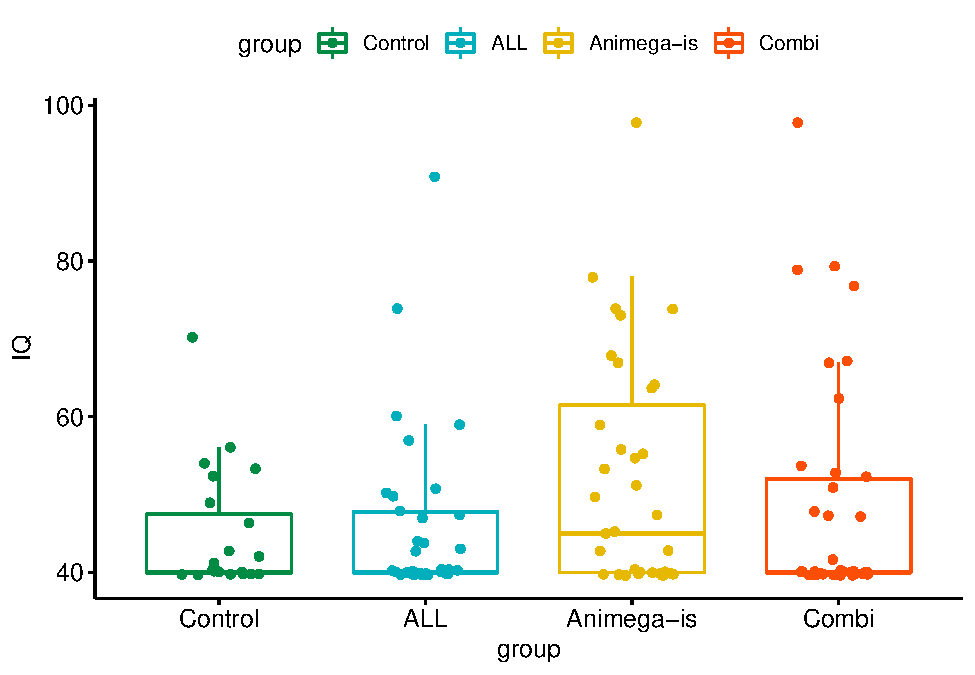
\includegraphics{Effects_of_training_files/figure-latex/IQ-plot-1.pdf}

\hypertarget{training-time-1}{%
\subsection{Training time}\label{training-time-1}}

The participants were instructed to train for a total of 18 hours (36 sessions for 30 minutes, three days a week for a 12-week period). The teachers were instructed to adapt the length of the training sessions after the need of the student. That is, if the student could not sit for a full 30 minute session the teacher was encouraged to have shorter sessions but more often than three times a week. On average the participants trained for 384.93 (\emph{sd} =194.12) minutes (6.42 (\emph{sd} =3.24) hours). There was no difference on training time between the three intervention groups (\emph{H}(2) = 0.57, \emph{p} =.751 ).

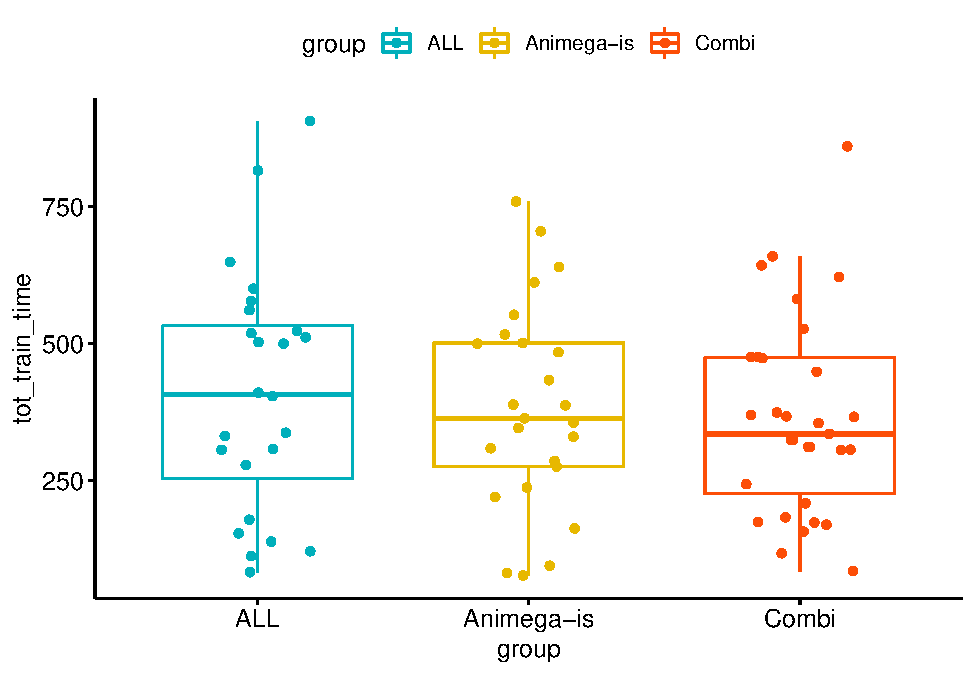
\includegraphics{Effects_of_training_files/figure-latex/tottraintime-plot-1.pdf}

\hypertarget{phonological-awareness}{%
\subsection{Phonological awareness}\label{phonological-awareness}}

\hypertarget{hypothesis-1a-training-phonemic-reading-strategies-improves-phonological-awareness.}{%
\subsubsection{Hypothesis 1a: Training phonemic reading strategies improves phonological awareness.}\label{hypothesis-1a-training-phonemic-reading-strategies-improves-phonological-awareness.}}

There was almost a significant interaction between time and the intervention on phonemic reading, the group training phonemic strategies improved more than the comparison group (\(\hat{\beta} = 0.01\), 95\% CI \([0.00, 0.02]\), \(t(362.23) = 1.66\), \(p = .097\)).

\hypertarget{hypothesis-1b-training-comprehension-based-reading-strategies-improves-phonological-awareness.}{%
\subsubsection{Hypothesis 1b: Training comprehension-based reading strategies improves phonological awareness.}\label{hypothesis-1b-training-comprehension-based-reading-strategies-improves-phonological-awareness.}}

There was no significant interaction between time and intervention for the comprehension-based reading strategy on PA (\(\hat{\beta} = 0.00\), 95\% CI \([0.00, 0.01]\), \(t(362.87) = 1.11\), \(p = .266\)).

\hypertarget{hypothesis-3-the-combined-training-is-more-effective-than-either-intervention-on-its-own.}{%
\subsubsection{Hypothesis 3: The combined training is more effective than either intervention on its own.}\label{hypothesis-3-the-combined-training-is-more-effective-than-either-intervention-on-its-own.}}

There was a significant interaction between the combined group and the other two intervention groups, (\(\hat{\beta} = 0.01\), 95\% CI \([0.00, 0.02]\), \(t(361.67) = 2.76\), \(p = .006\)), the combined training improved PA over time more than the other two intervention groups.

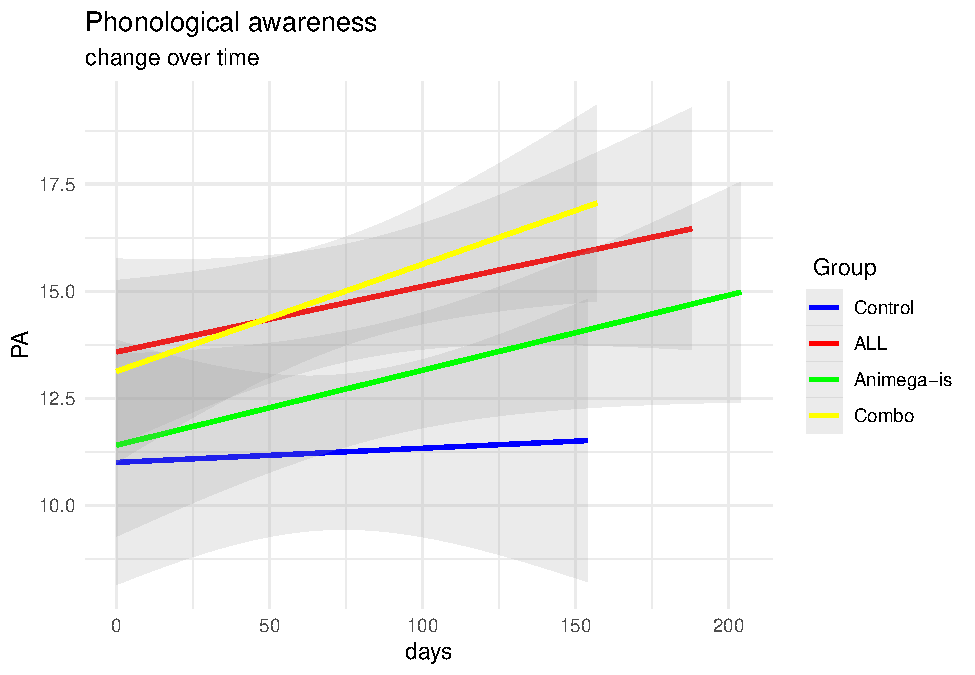
\includegraphics{Effects_of_training_files/figure-latex/PA-plot-1.pdf}

\hypertarget{exploratory-analyses}{%
\subsection{Exploratory analyses}\label{exploratory-analyses}}

\hypertarget{effect-of-iq}{%
\subsubsection{Effect of IQ}\label{effect-of-iq}}

There was a significant main effect on IQ (\(\hat{\beta} = 1.69\), 95\% CI \([0.37, 3.02]\), \(t(156.06) = 2.51\), \(p = .013\)), indicating that higher IQ results in higher PA at T1. Moreover, there was a significant interaction between time and IQ (\(\hat{\beta} = 0.01\), 95\% CI \([0.00, 0.01]\), \(t(357.34) = 2.46\), \(p = .014\)), indicating that the participants with the highest IQ benefited the most from the intervention. However, the benefit of the combined training over the two other intervention types remained (\(\hat{\beta} = 0.01\), 95\% CI \([0.00, 0.02]\), \(t(355.72) = 2.83\), \(p = .005\))

The results from the PA models can be seen in Table~\ref{tab:PA-table}.

~

PA

PA

Predictors

Estimates

CI

p

df

Estimates

CI

p

df

(Intercept)

12.24

10.94~--~13.54

\textless0.001

483.00

12.45

11.13~--~13.77

\textless0.001

469.00

days

0.01

0.01~--~0.02

\textless0.001

483.00

0.01

0.01~--~0.02

\textless0.001

469.00

contrast 1vs2

1.79

-0.37~--~3.95

0.104

483.00

1.66

-0.51~--~3.84

0.134

469.00

contrast 1vs3

-0.30

-2.44~--~1.85

0.787

483.00

-1.17

-3.39~--~1.05

0.301

469.00

contrast 4vs23

0.82

-1.39~--~3.02

0.467

483.00

0.48

-1.70~--~2.67

0.663

469.00

days * contrast 1vs2

0.01

-0.00~--~0.02

0.097

483.00

0.01

-0.00~--~0.02

0.057

469.00

days * contrast 1vs3

0.00

-0.00~--~0.01

0.266

483.00

0.00

-0.01~--~0.01

0.628

469.00

days * contrast 4vs23

0.01

0.00~--~0.02

0.006

483.00

0.01

0.00~--~0.02

0.005

469.00

IQ scale

1.69

0.37~--~3.02

0.012

469.00

days * IQ scale

0.01

0.00~--~0.01

0.014

469.00

Random Effects

σ2

12.38

12.18

τ00

49.69 id

46.87 id

ICC

0.80

0.79

N

135 id

128 id

Observations

493

481

Marginal R2 / Conditional R2

0.056 / 0.812

0.113 / 0.817

\hypertarget{word-reading}{%
\subsection{Word reading}\label{word-reading}}

\hypertarget{hypothesis-1a-training-phonemic-reading-strategies-improves-word-reading.}{%
\subsubsection{Hypothesis 1a: Training phonemic reading strategies improves word reading.}\label{hypothesis-1a-training-phonemic-reading-strategies-improves-word-reading.}}

There was not a significant interaction between time and the intervention on phonemic-based reading (\(\hat{\beta} = 0.05\), 95\% CI \([-0.05, 0.16]\), \(t(130.31) = 0.95\), \(p = .344\)).

\hypertarget{hypothesis-1b-training-comprehension-based-reading-strategies-improves-word-awareness.}{%
\subsubsection{Hypothesis 1b: Training comprehension-based reading strategies improves word awareness.}\label{hypothesis-1b-training-comprehension-based-reading-strategies-improves-word-awareness.}}

There was no significant interaction between time and intervention for the comprehension-based reading strategy on word reading (\(\hat{\beta} = 0.00\), 95\% CI \([-0.10, 0.10]\), \(t(117.46) = 0.04\), \(p = .970\)).

\hypertarget{hypothesis-3-the-combined-training-is-more-effective-than-either-intervention-on-its-own.-1}{%
\subsubsection{Hypothesis 3: The combined training is more effective than either intervention on its own.}\label{hypothesis-3-the-combined-training-is-more-effective-than-either-intervention-on-its-own.-1}}

There was a not significant interaction between the combined group and the other two intervention groups, (\(\hat{\beta} = -0.01\), 95\% CI \([-0.13, 0.10]\), \(t(165.26) = -0.21\), \(p = .836\)).

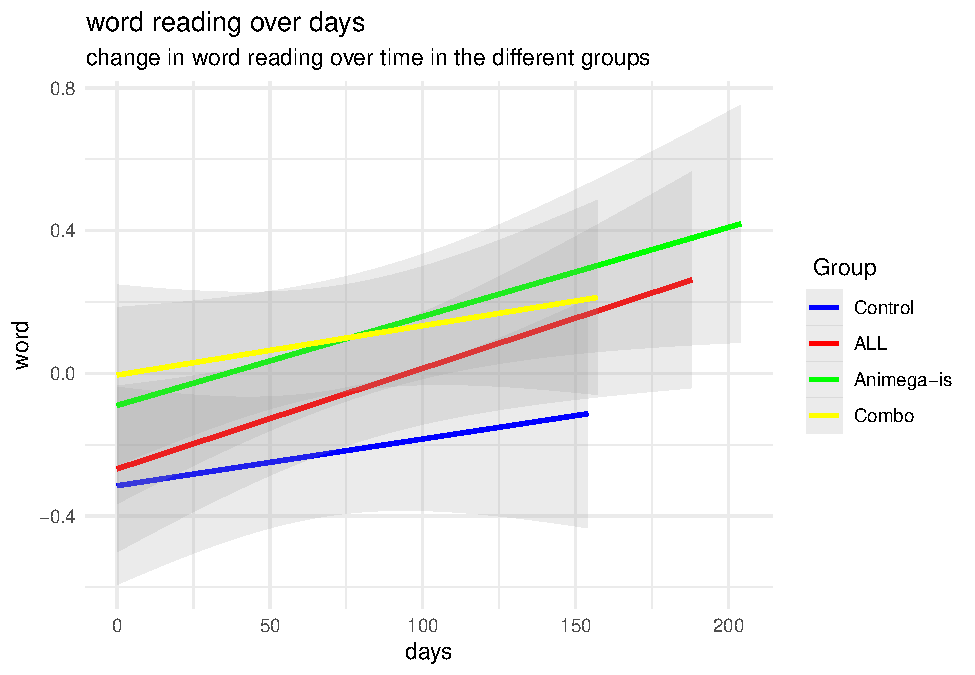
\includegraphics{Effects_of_training_files/figure-latex/word-plot-1.pdf}

\hypertarget{exploratory-analyses-1}{%
\subsection{Exploratory analyses}\label{exploratory-analyses-1}}

\hypertarget{effect-of-iq-1}{%
\subsubsection{Effect of IQ}\label{effect-of-iq-1}}

There was a significant main effect on IQ (\(\hat{\beta} = 0.16\), 95\% CI \([0.01, 0.30]\), \(t(128.40) = 2.15\), \(p = .034\)), indicating that higher IQ results in higher word reading at T1. Moreover, there was a significant interaction between time and IQ (\(\hat{\beta} = 0.06\), 95\% CI \([0.00, 0.13]\), \(t(114.71) = 1.99\), \(p = .049\)), indicating that the participants with the highest IQ improved most over the training period regardless of intervention condition (including control).

\hypertarget{effect-of-pa}{%
\subsubsection{Effect of PA}\label{effect-of-pa}}

There was a significant main effect on PA (\(\hat{\beta} = 0.30\), 95\% CI \([0.21, 0.38]\), \(t(476.03) = 6.66\), \(p < .001\)), indicating that higher PA resulted in higher word reading at T1. Moreover, there was a significant interaction between time and PA (), indicating that the participants with the highest PA improved most over the training period regardless of intervention condition (including control).

The results from the word models can be seen in Table~\ref{tab:word-table}.

~

word

word

word

Predictors

Estimates

CI

p

df

Estimates

CI

p

df

Estimates

CI

p

df

(Intercept)

-0.18

-0.32~--~-0.05

0.009

477.00

-0.18

-0.32~--~-0.04

0.014

463.00

-0.13

-0.25~--~-0.01

0.029

463.00

days

0.20

0.14~--~0.27

\textless0.001

477.00

0.20

0.14~--~0.27

\textless0.001

463.00

0.14

0.07~--~0.20

\textless0.001

463.00

contrast 1vs2

0.00

-0.23~--~0.23

0.991

477.00

0.01

-0.23~--~0.24

0.939

463.00

-0.06

-0.25~--~0.14

0.573

463.00

contrast 1vs3

0.15

-0.07~--~0.38

0.181

477.00

0.09

-0.14~--~0.33

0.435

463.00

0.14

-0.05~--~0.34

0.152

463.00

contrast 4vs23

0.16

-0.07~--~0.39

0.178

477.00

0.14

-0.09~--~0.38

0.228

463.00

0.13

-0.06~--~0.32

0.191

463.00

days * contrast 1vs2

0.05

-0.05~--~0.16

0.342

477.00

0.06

-0.04~--~0.17

0.243

463.00

0.00

-0.10~--~0.11

0.935

463.00

days * contrast 1vs3

0.00

-0.10~--~0.10

0.970

477.00

-0.02

-0.12~--~0.08

0.706

463.00

-0.03

-0.13~--~0.07

0.594

463.00

days * contrast 4vs23

-0.01

-0.13~--~0.10

0.836

477.00

-0.01

-0.12~--~0.10

0.864

463.00

-0.09

-0.20~--~0.02

0.117

463.00

IQ scale

0.16

0.01~--~0.30

0.032

463.00

0.09

-0.03~--~0.21

0.132

463.00

days * IQ scale

0.06

0.00~--~0.13

0.047

463.00

0.01

-0.05~--~0.08

0.655

463.00

PA

0.30

0.21~--~0.38

\textless0.001

463.00

days * PA

0.09

0.03~--~0.15

0.006

463.00

Random Effects

σ2

0.15

0.15

0.16

τ00

0.54 id

0.53 id

0.32 id

τ11

0.02 id.scale(days, center = FALSE)

0.02 id.scale(days, center = FALSE)

~

ρ01

0.46 id

0.48 id

~

ICC

0.81

0.80

0.66

N

134 id

127 id

127 id

Observations

489

477

477

Marginal R2 / Conditional R2

0.041 / 0.820

0.087 / 0.819

0.287 / 0.759

\hypertarget{sentence-reading}{%
\section{Sentence reading}\label{sentence-reading}}

\hypertarget{hypothesis-1a-training-phonemic-reading-strategies-improves-sentence-reading.}{%
\subsubsection{Hypothesis 1a: Training phonemic reading strategies improves sentence reading.}\label{hypothesis-1a-training-phonemic-reading-strategies-improves-sentence-reading.}}

There was not a significant interaction between time and the intervention on phonemic training on sentence reading (\(\hat{\beta} = 0.19\), 95\% CI \([-0.24, 0.61]\), \(z = 0.86\), \(p = .392\)).

\hypertarget{hypothesis-1b-training-comprehension-based-reading-strategies-improves-sentence-awareness.}{%
\subsubsection{Hypothesis 1b: Training comprehension-based reading strategies improves sentence awareness.}\label{hypothesis-1b-training-comprehension-based-reading-strategies-improves-sentence-awareness.}}

There was no significant interaction between time and intervention for the comprehension-based reading strategy on sentence reading (\(\hat{\beta} = -0.09\), 95\% CI \([-0.51, 0.32]\), \(z = -0.44\), \(p = .659\)).

\hypertarget{hypothesis-3-the-combined-training-is-more-effective-than-either-intervention-on-its-own.-2}{%
\subsubsection{Hypothesis 3: The combined training is more effective than either intervention on its own.}\label{hypothesis-3-the-combined-training-is-more-effective-than-either-intervention-on-its-own.-2}}

There was a not significant interaction between the combined group and the other two intervention groups, (\(\hat{\beta} = -0.12\), 95\% CI \([-0.63, 0.39]\), \(z = -0.47\), \(p = .641\)).

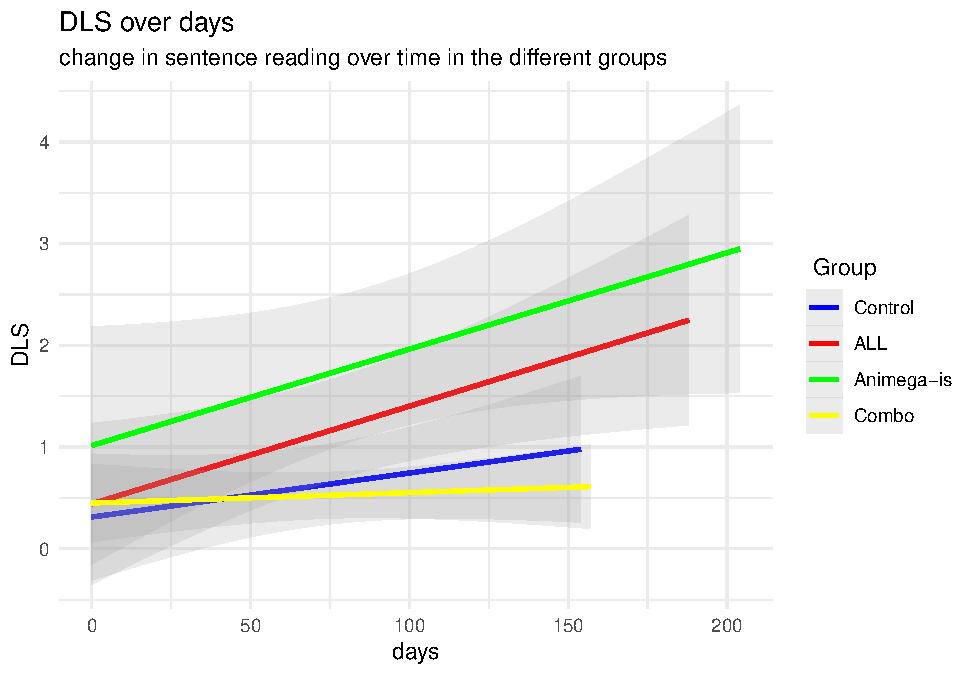
\includegraphics{Effects_of_training_files/figure-latex/DLS-plot-1.pdf}

\hypertarget{exploratory-analyses-2}{%
\subsection{Exploratory analyses}\label{exploratory-analyses-2}}

\hypertarget{effect-of-iq-2}{%
\subsubsection{Effect of IQ}\label{effect-of-iq-2}}

There was a significant main effect on IQ (\(\hat{\beta} = 0.50\), 95\% CI \([-0.13, 1.13]\), \(z = 1.57\), \(p = .117\)), indicating that higher IQ results in higher sentence reading at T1. Moreover, there was a significant interaction between time and IQ (\(\hat{\beta} = 0.18\), 95\% CI \([-0.09, 0.45]\), \(z = 1.32\), \(p = .188\)), indicating that the participants with the highest IQ improved most over the training period regardless of intervention condition (including control).

\hypertarget{effect-of-pa-1}{%
\subsubsection{Effect of PA}\label{effect-of-pa-1}}

There was a significant main effect on PA (\(\hat{\beta} = 0.87\), 95\% CI \([0.52, 1.23]\), \(z = 4.79\), \(p < .001\)), indicating that higher PA resulted in higher word reading at T1. However, there was not a significant interaction between time and PA (\(\hat{\beta} = 0.00\), 95\% CI \([-0.24, 0.25]\), \(z = 0.04\), \(p = .968\)), indicating that the participants' PA did not affect the improvement rate over the training period.

The results from the word models can be seen in Table~\ref{tab:DLS-table}.

~

DLS

DLS

DLS

Predictors

Incidence Rate Ratios

CI

p

Incidence Rate Ratios

CI

p

Incidence Rate Ratios

CI

p

(Intercept)

0.07

0.03~--~0.14

\textless0.001

0.03

0.01~--~0.10

\textless0.001

0.11

0.06~--~0.19

\textless0.001

days

1.72

1.27~--~2.33

\textless0.001

3.22

1.66~--~6.26

0.001

1.43

1.08~--~1.90

0.012

contrast 1vs2

1.07

0.45~--~2.55

0.877

contrast 1vs3

1.38

0.59~--~3.24

0.463

contrast 4vs23

0.84

0.34~--~2.08

0.711

days * contrast 1vs2

1.20

0.79~--~1.85

0.392

days * contrast 1vs3

0.91

0.60~--~1.38

0.659

days * contrast 4vs23

0.89

0.53~--~1.47

0.641

IQ scale

1.65

0.88~--~3.10

0.117

1.24

0.84~--~1.85

0.281

IQ scale * days

1.20

0.91~--~1.58

0.188

1.23

1.06~--~1.44

0.008

PA

2.39

1.67~--~3.42

\textless0.001

days * PA

1.01

0.79~--~1.28

0.968

Random Effects

σ2

2.42

2.49

2.23

τ00

5.42 id

7.94 id

2.73 id

τ11

0.40 id.scale(days, center = FALSE)

0.52 id.scale(days, center = FALSE)

~

ρ01

~

-0.74 id

~

ICC

0.69

0.71

0.55

N

134 id

127 id

127 id

Observations

488

476

476

Marginal R2 / Conditional R2

0.034 / 0.702

0.102 / 0.739

0.195 / 0.638

\hypertarget{explorative-analyses}{%
\section{Explorative analyses}\label{explorative-analyses}}

\hypertarget{letter-sound-recognition}{%
\subsection{Letter-sound recognition}\label{letter-sound-recognition}}

\hypertarget{hypothesis-1a-training-phonemic-reading-strategies-improves-letter-sound-recognition.}{%
\subsubsection{Hypothesis 1a: Training phonemic reading strategies improves letter-sound recognition.}\label{hypothesis-1a-training-phonemic-reading-strategies-improves-letter-sound-recognition.}}

There was a significant interaction between time and the intervention on phonemic training on sentence reading (\(\hat{\beta} = 0.43\), 95\% CI \([0.13, 0.74]\), \(t(124.39) = 2.82\), \(p = .006\)).

\hypertarget{hypothesis-1b-training-comprehension-based-reading-strategies-improves-sletter-sound-recognition.}{%
\subsubsection{Hypothesis 1b: Training comprehension-based reading strategies improves sletter-sound recognition.}\label{hypothesis-1b-training-comprehension-based-reading-strategies-improves-sletter-sound-recognition.}}

There was no significant interaction between time and intervention for the comprehension-based reading strategy on sentence reading (\(\hat{\beta} = 0.07\), 95\% CI \([-0.22, 0.36]\), \(t(112.37) = 0.46\), \(p = .645\)).

\hypertarget{hypothesis-3-the-combined-training-is-more-effective-than-either-intervention-on-its-own.-3}{%
\subsubsection{Hypothesis 3: The combined training is more effective than either intervention on its own.}\label{hypothesis-3-the-combined-training-is-more-effective-than-either-intervention-on-its-own.-3}}

There was a not significant interaction between the combined group and the other two intervention groups, (\(\hat{\beta} = 0.06\), 95\% CI \([-0.26, 0.39]\), \(t(159.28) = 0.38\), \(p = .705\)).

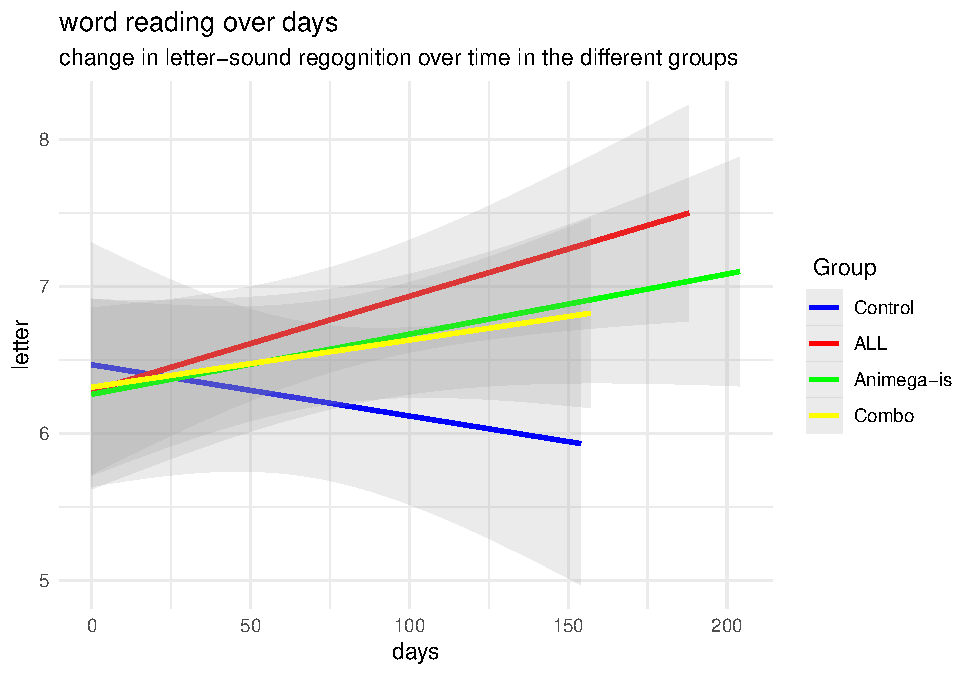
\includegraphics{Effects_of_training_files/figure-latex/letter-plot-1.pdf}

\hypertarget{effect-of-iq-3}{%
\subsubsection{Effect of IQ}\label{effect-of-iq-3}}

There was a significant main effect on IQ (\(\hat{\beta} = 0.51\), 95\% CI \([0.08, 0.93]\), \(t(129.19) = 2.32\), \(p = .022\)), indicating that higher IQ results in higher sentence reading at T1. However, there was not a significant interaction between time and IQ (\(\hat{\beta} = -0.11\), 95\% CI \([-0.30, 0.08]\), \(t(112.06) = -1.12\), \(p = .263\)), indicating that the participants' IQ did not affect the improvement rate over the training period.

\hypertarget{effect-of-pa-2}{%
\subsubsection{Effect of PA}\label{effect-of-pa-2}}

There was a significant main effect on PA (\(\hat{\beta} = 0.92\), 95\% CI \([0.65, 1.19]\), \(t(255.81) = 6.72\), \(p < .001\)), indicating that higher PA resulted in higher word reading at T1. Moreover, there was a significant interaction between time and PA (), indicating that the participants with the highest PA improved most over the training period regardless of intervention condition (including control).

The results from the word models can be seen in Table~\ref{tab:letter-table}.

~

letter

letter

letter

Predictors

Estimates

CI

p

df

Estimates

CI

p

df

Estimates

CI

p

df

(Intercept)

6.29

5.88~--~6.70

\textless0.001

482.00

6.30

5.87~--~6.72

\textless0.001

468.00

6.44

6.09~--~6.80

\textless0.001

465.00

days

0.23

0.05~--~0.42

0.015

482.00

0.24

0.05~--~0.43

0.015

468.00

0.10

-0.10~--~0.29

0.349

465.00

contrast 1vs2

-0.05

-0.73~--~0.63

0.883

482.00

0.00

-0.70~--~0.71

0.992

468.00

-0.19

-0.77~--~0.39

0.527

465.00

contrast 1vs3

-0.09

-0.77~--~0.60

0.806

482.00

-0.27

-0.99~--~0.45

0.462

468.00

-0.13

-0.72~--~0.46

0.671

465.00

contrast 4vs23

-0.00

-0.70~--~0.69

0.997

482.00

-0.04

-0.74~--~0.67

0.920

468.00

-0.07

-0.65~--~0.51

0.805

465.00

days * contrast 1vs2

0.43

0.13~--~0.74

0.005

482.00

0.41

0.10~--~0.72

0.009

468.00

0.36

0.04~--~0.68

0.029

465.00

days * contrast 1vs3

0.07

-0.22~--~0.36

0.644

482.00

0.10

-0.21~--~0.41

0.525

468.00

0.07

-0.24~--~0.39

0.644

465.00

days * contrast 4vs23

0.06

-0.26~--~0.39

0.705

482.00

0.07

-0.26~--~0.40

0.694

468.00

-0.05

-0.39~--~0.29

0.752

465.00

IQ scale

0.51

0.08~--~0.93

0.021

468.00

0.30

-0.06~--~0.66

0.101

465.00

days * IQ scale

-0.11

-0.30~--~0.08

0.261

468.00

-0.14

-0.34~--~0.05

0.155

465.00

PA

0.92

0.65~--~1.19

\textless0.001

465.00

days * PA

-0.12

-0.31~--~0.07

0.225

465.00

Random Effects

σ2

1.22

1.23

1.26

τ00

5.00 id

4.94 id

3.03 id

τ11

0.24 id.scale(days, center = FALSE)

0.24 id.scale(days, center = FALSE)

0.28 id.scale(days, center = FALSE)

ρ01

-0.79 id

-0.80 id

-0.70 id

ICC

0.76

0.76

0.65

N

136 id

129 id

128 id

Observations

494

482

481

Marginal R2 / Conditional R2

0.018 / 0.765

0.048 / 0.767

0.199 / 0.716

\hypertarget{marginal-and-conditional-r2}{%
\section{marginal and conditional R2}\label{marginal-and-conditional-r2}}

A marginal R2 close to zero tells us that the fixed effects aren't explaining much variation, and a conditional R2 close to 1 tells us that most of that unexplained variation is between groups (people) rather than between observations within groups (people). So, for example, if the context was a longitudinal cohort study, we wouldn't expect to improve our model much by collecting more data on characteristics/measures that mainly vary within people, but instead should find characteristics that mainly vary between people.

\#Ska vi även redovisa om Animega-is var bättre än de andra grupperna på letter-sound recognition? - De var de inte.

\hypertarget{results-summary}{%
\section{Results summary}\label{results-summary}}

Combination group improves more on PA compared to the other intervention groups. PA intervention improves letter-sound recognition more than other intervention groups. IQ influences improvement over time on many outcome measures (sammanfatta vilka här). PA interacts with time on letter-sound recognition, word reading and sentence reading, suggesting that PA predicts improvement in those outcome variables.

\hypertarget{discussion}{%
\section{Discussion}\label{discussion}}

Blablablablalba

\#\#Conclusions
Blablabla

\#\#Declaration of interest
Blablabla

\newpage

\hypertarget{references}{%
\section{References}\label{references}}

\begingroup
\setlength{\parindent}{-0.5in}
\setlength{\leftskip}{0.5in}

\hypertarget{refs}{}
\begin{CSLReferences}{1}{0}
\leavevmode\vadjust pre{\hypertarget{ref-R-papaja}{}}%
Aust, F., \& Barth, M. (2018). \emph{{papaja}: {Create} {APA} manuscripts with {R Markdown}}. Retrieved from \url{https://github.com/crsh/papaja}

\leavevmode\vadjust pre{\hypertarget{ref-R-lme4}{}}%
Bates, D., Mächler, M., Bolker, B., \& Walker, S. (2015). Fitting linear mixed-effects models using {lme4}. \emph{Journal of Statistical Software}, \emph{67}(1), 1--48. \url{https://doi.org/10.18637/jss.v067.i01}

\leavevmode\vadjust pre{\hypertarget{ref-R-Matrix}{}}%
Bates, D., \& Maechler, M. (2018). \emph{Matrix: Sparse and dense matrix classes and methods}. Retrieved from \url{https://CRAN.R-project.org/package=Matrix}

\leavevmode\vadjust pre{\hypertarget{ref-Facon2011}{}}%
Facon, B., Magis, D., \& Belmont, J. M. (2011). {Beyond matching on the mean in developmental disabilities research}. \emph{Research in Developmental Disabilities}, \emph{32}(6), 2134--2147. \url{https://doi.org/10.1016/j.ridd.2011.07.029}

\leavevmode\vadjust pre{\hypertarget{ref-R-base}{}}%
R Core Team. (2018). \emph{R: A language and environment for statistical computing}. Vienna, Austria: R Foundation for Statistical Computing. Retrieved from \url{https://www.R-project.org/}

\leavevmode\vadjust pre{\hypertarget{ref-R-ggplot2}{}}%
Wickham, H. (2016). \emph{ggplot2: Elegant graphics for data analysis}. Springer-Verlag New York. Retrieved from \url{https://ggplot2.tidyverse.org}

\leavevmode\vadjust pre{\hypertarget{ref-R-dplyr}{}}%
Wickham, H., François, R., Henry, L., \& Müller, K. (2018). \emph{Dplyr: A grammar of data manipulation}. Retrieved from \url{https://CRAN.R-project.org/package=dplyr}

\leavevmode\vadjust pre{\hypertarget{ref-R-tidyr}{}}%
Wickham, H., \& Henry, L. (2018). \emph{Tidyr: Easily tidy data with 'spread()' and 'gather()' functions}. Retrieved from \url{https://CRAN.R-project.org/package=tidyr}

\leavevmode\vadjust pre{\hypertarget{ref-WorldMedicalAssociation2013}{}}%
World Medical Association. (2013). {World Medical Association Declaration of Helsinki}. \emph{JAMA}, \emph{310}(20), 2191. \url{https://doi.org/10.1001/jama.2013.281053}

\end{CSLReferences}

\endgroup


\end{document}
